\documentclass{beamer}

\usepackage{graphicx}
\usepackage{algorithmic}
\usepackage{amsmath}
\usepackage{amsfonts}
\usepackage{amssymb}
\usepackage{amsthm}
\usepackage[abs]{overpic}
\usepackage{pict2e}
\usepackage[absolute,overlay]{textpos}
\usepackage{algorithmic}
\usepackage{amsfonts}
\usepackage{amsmath}
\usepackage{amssymb}
\usepackage{bbm}
\usepackage{bm}
\usepackage{color}
\usepackage{comment}
\usepackage{enumerate}
\usepackage{epsfig}
\usepackage{exscale}
\usepackage{framed}
\usepackage{graphicx}
\usepackage{rotating}
\usepackage{latexsym}
\usepackage{float}
\usepackage{mdwlist}
\usepackage{microtype}
\usepackage{multirow}
\usepackage{xmpmulti,multimedia,xspace}

\usepackage{algorithm}
\usepackage{algorithmic}

\newcommand{\explain}[2]{\underbrace{#2}_{\mbox{\footnotesize{#1}}}}





\let\oldframetitle\frametitle
\renewcommand{\frametitle}[1]{
\oldframetitle{#1}
\BottomLogo
}

\let\oldtitlepage\titlepage
\renewcommand{\titlepage}{
\oldtitlepage
\TitleLogo
}
\setlength{\TPHorizModule}{1mm}
\setlength{\TPVertModule}{1mm}

\newcommand{\TopLogo}{
\begin{textblock}{14}(70.0,2.0)

\includegraphics[height=.8cm]{figures/umd-logo2.jpg}
\end{textblock}
}
\newcommand{\BottomLogo}{
\begin{textblock}{14}(118.0,84.0)

\includegraphics[height=.8cm]{figures/umd-logo1.jpg}
\end{textblock}
}
\newcommand{\TitleLogo}{
\begin{textblock}{14}(2.0,3.0)

\includegraphics[height=1.0cm]{figures/umd-logo2.jpg}
\end{textblock}
}




\def\simiid{\stackrel{\rm i.i.d.}{\sim}}
\def\Bet{\mbox{Beta}}
\def\Poi{\mbox{Poisson}}


\mode<presentation>
{
  
  \usetheme{Madrid} 
  
  
  
  
  
  
  
  
  
  
  
  
  
  
  
  
  
  

  
  
}
\setbeamertemplate{navigation symbols}{}



\usecolortheme[rgb={0.2, 0.2, 0.6}]{structure}









\title[Spectral Algorithms for Topic Models]{Spectral Algorithms for Topic Models: An Evaluation}


\author[Thang Nguyen et al.] {Thang Nguyen, Peratham Wiriyathammabhum, \\ Yuening Hu, Jordan Boyd-Graber}

\institute[UMD]{

   {daithang,peratham,ynhu,jbg}@umiacs.umd.edu\\
   University of Maryland, College Park
}
\date{Oct. 11, 2013}







\begin{document}
\begin{frame}
  \titlepage
\end{frame}

\begin{frame}
\frametitle{Introduction}

\begin{itemize}
\item Topic models
\begin{itemize}
\item Unsupervised methods that learn thematic structures from a set of documents
\item Each document is an admixture over a distribution over topics
\item Typical topic discovery includes MCMC or variational EM
\item Easy to get trapped to local optima
\item Iterative learning, hard to decide whether converged or not
\end{itemize}

\item Recent spectral algorithms for topic models
\begin{itemize}
\item Such as {\bf anchor} method (Arora et al., 2012) and moment-based method (Anandkumar et al, 2012)
\item Provable polynomial-time solutions
\item Not flexible enough to incorporate the rich priors of topic models
\item Have not been evaluated using traditional topic model evaluations
\end{itemize}
\end{itemize}
\end{frame}


\begin{frame}
\frametitle{Anchor Algorithm (Arora et al., 2012)}
\begin{itemize}
\item Separability Assumption
\begin{itemize}
\item Every topic contains at least one anchor word: positive probability only for this topic, 0 for others topics
\item A document contains an anchor word will be guaranteed that it contain this anchor word's corresponding topic
\item Hence faster inference mechanism
\end{itemize}
\item Two steps:
\begin{itemize}
\item Anchor word selection: select anchor words from a pool of anchor candidates (word appears more than $M$ documents)
\item Recover topic distributions given those anchor words
\end{itemize}
\end{itemize} 
\end{frame}

\begin{frame}
\frametitle{Anchor Algorithm: recovery step}
\begin{itemize}
\item Let $Q$ denote the input word co-occurrence matrix; $\bar{Q}$ denote the
row-normalized $Q$; the indices of anchor words as $S = {s_1, s_2,
  \cdots, s_K}$; $Q(s_k)$ as the conditional cooccurence probability of anchor
words for topic $k$; $C_{i,k} = p(z=k|w=i)$.  This induces an objective
\begin{equation}
\label{eq:anchor}
C_i. = argmin_{\vec{C_i}} D_{KL}(\bar{Q}_i || \sum_{k\in S} C_{i,k} \bar{Q}_{s_k})
\end{equation}

\item We inject prior knowledge by adding different regularization on $\hat C$ matrix, instead of just considering
the KL divergence in Equation~\ref{eq:anchor}
\end{itemize}
\end{frame}

\begin{frame}
\frametitle{Regularized Algorithms}
\begin{itemize}
\item {\bf L2 Norm} regularization (Gaussian Prior)
\begin{equation}
\label{eq:anchorl2}
C_i. = argmin_{\vec{C_i}} D_{KL}(\bar{Q}_i || \sum_{k\in S} C_{i,k} \bar{Q}_{s_k}) +\lambda \|C_i\| \notag
\end{equation}

\item {\bf Beta Norm} regularization (Dirichlet Prior)
\begin{equation}
\label{eq:anchorbeta}
C_i. = argmin_{\vec{C_i}}D_{KL}(\bar{Q}_i \| \sum_{k \in S} C_{i,k} \bar{Q}_{s_k})- \lambda \sum_{k\in S}\mbox{log (Beta}(\beta_{k,i};\alpha,(V-1)\alpha)) \notag
\end{equation}

\begin{itemize}
\item $\beta_{k,i} = p(w=i|z=k), \mbox{$i \in V$ and $k \in S$}$
\item Beta($\beta;a,b$) is the Beta function
\item $V$ is the size of vocabulary
\item $\lambda$ is the regularization term
\item $\alpha$ is the Dirichlet term for topic model (usually = $\frac{60}{V}$)
\end{itemize}
\end{itemize}
\end{frame}


\begin{frame}
\frametitle{Evaluation Measures}
\begin{itemize}
\item Held-out likelihood (Blei et al., 2003)
\begin{itemize}
\item How much the model generalizes on held-out documents
\item Use implementation of LDAC inference
\end{itemize}

\item Topic Interpretability (Chang et al., 2009; Newman et al., 2010)
\begin{itemize}
\item Tells us how "readable" and "interpretable" the output topics generated by a topic modeling algorithm
\item Use Normalized Pointwise Mutual Information (NPMI)
\end{itemize}

\item Use grid search to find $M$ and regularization term $\lambda$
\end{itemize}
\end{frame}

\begin{frame}
\frametitle{Datasets}

\begin{itemize}
\item 20NewsGroup dataset
\begin{itemize}
\item TRAIN set: 11243 documents (70\%)
\item DEV set: 3748 documents (15\%)
\item TEST set: 3740 documents (15\%)
\item Vocabulary size: 81600 terms
\end{itemize}

\item NIPS dataset
\begin{itemize}
\item TRAIN set: 1039 documents (70\%)
\item DEV set: 228 documents (15\%)
\item TEST set: 233 documents (15\%)
\item Vocabulary size: 12182 terms
\end{itemize}

\end{itemize}
\end{frame}



















\begin{frame}

\frametitle{NIPS Data Result: Tuning Set, M=100}

\begin{figure}
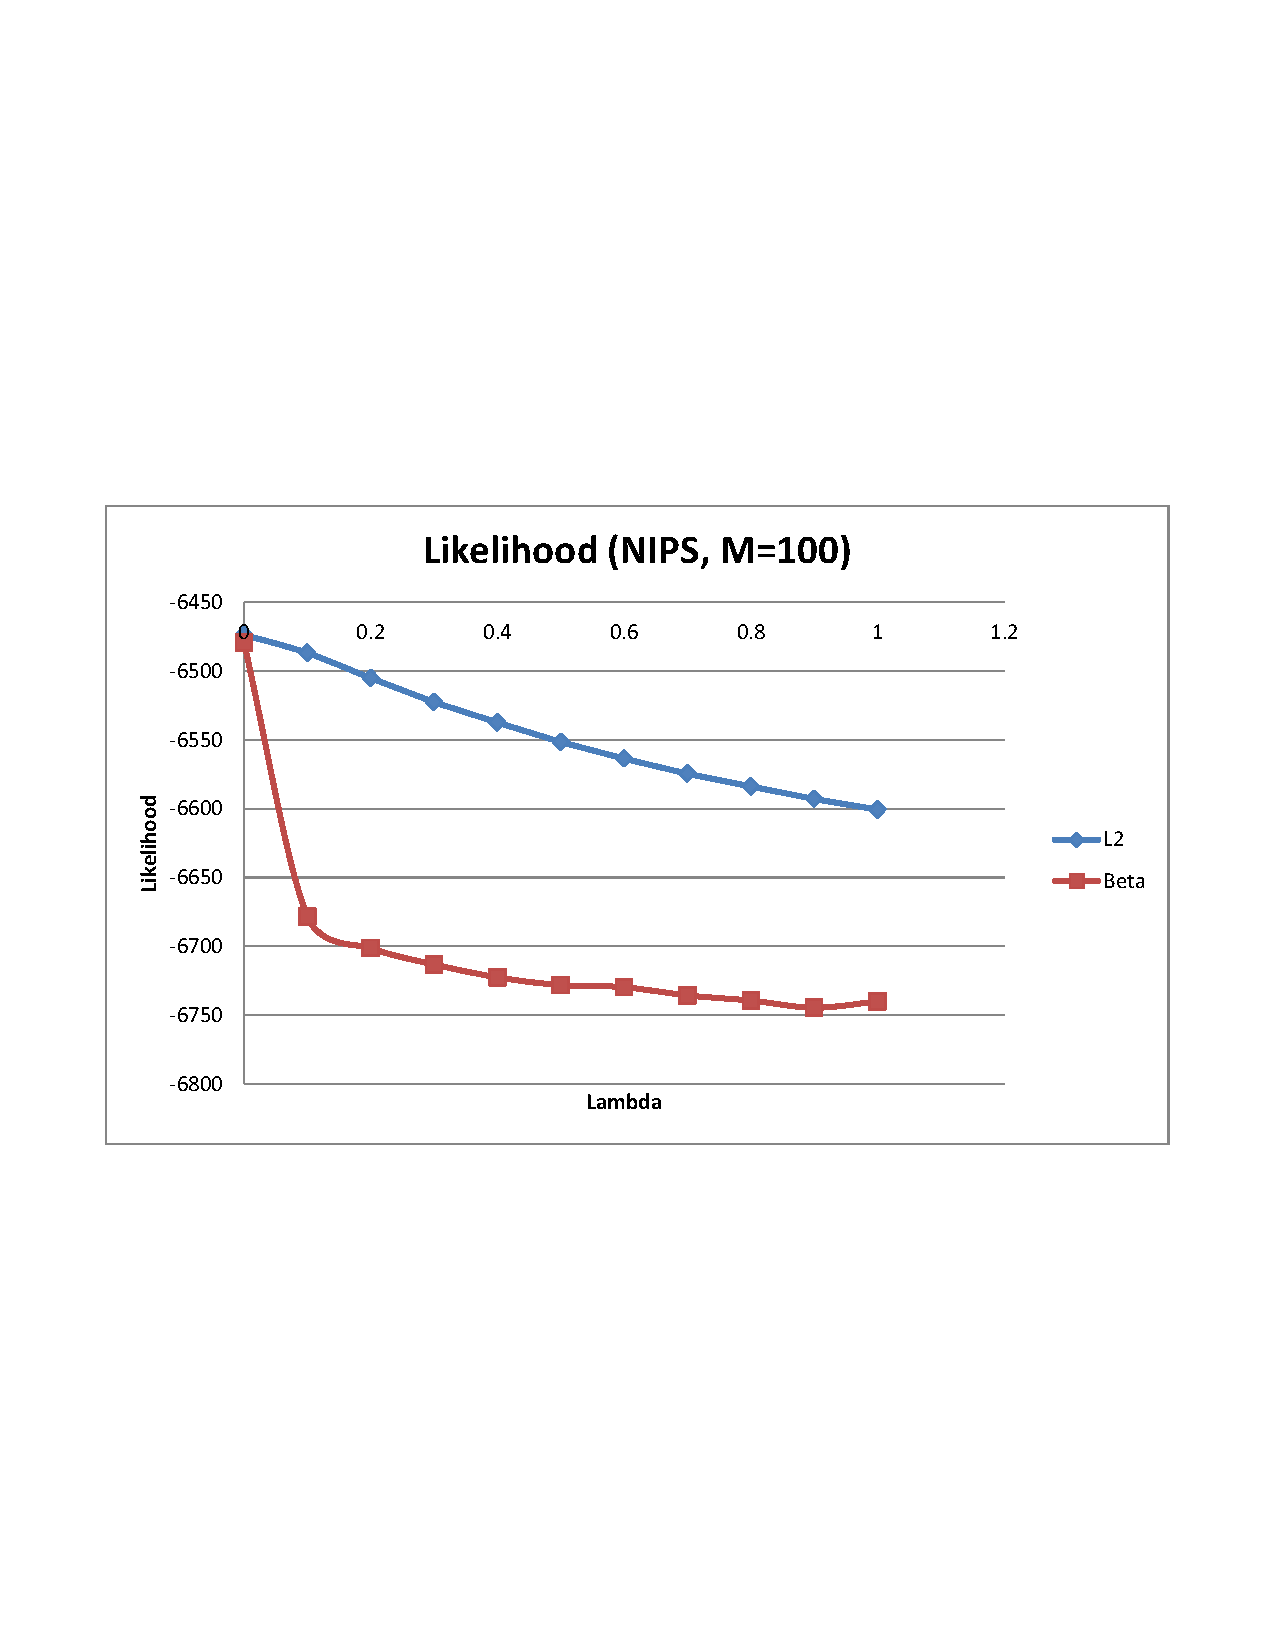
\includegraphics[width=0.7\linewidth]{figures/NIPS_M_100_Likelihood.pdf}
\end{figure}
\vspace{-0.1in}
\begin{itemize}
\item Both L2 Norm and Beta norm performs worse than original {\bf anchor} on Held-out score
\end{itemize}
\end{frame} 

\begin{frame}
\frametitle{NIPS Data Result: M=100}
\begin{figure}
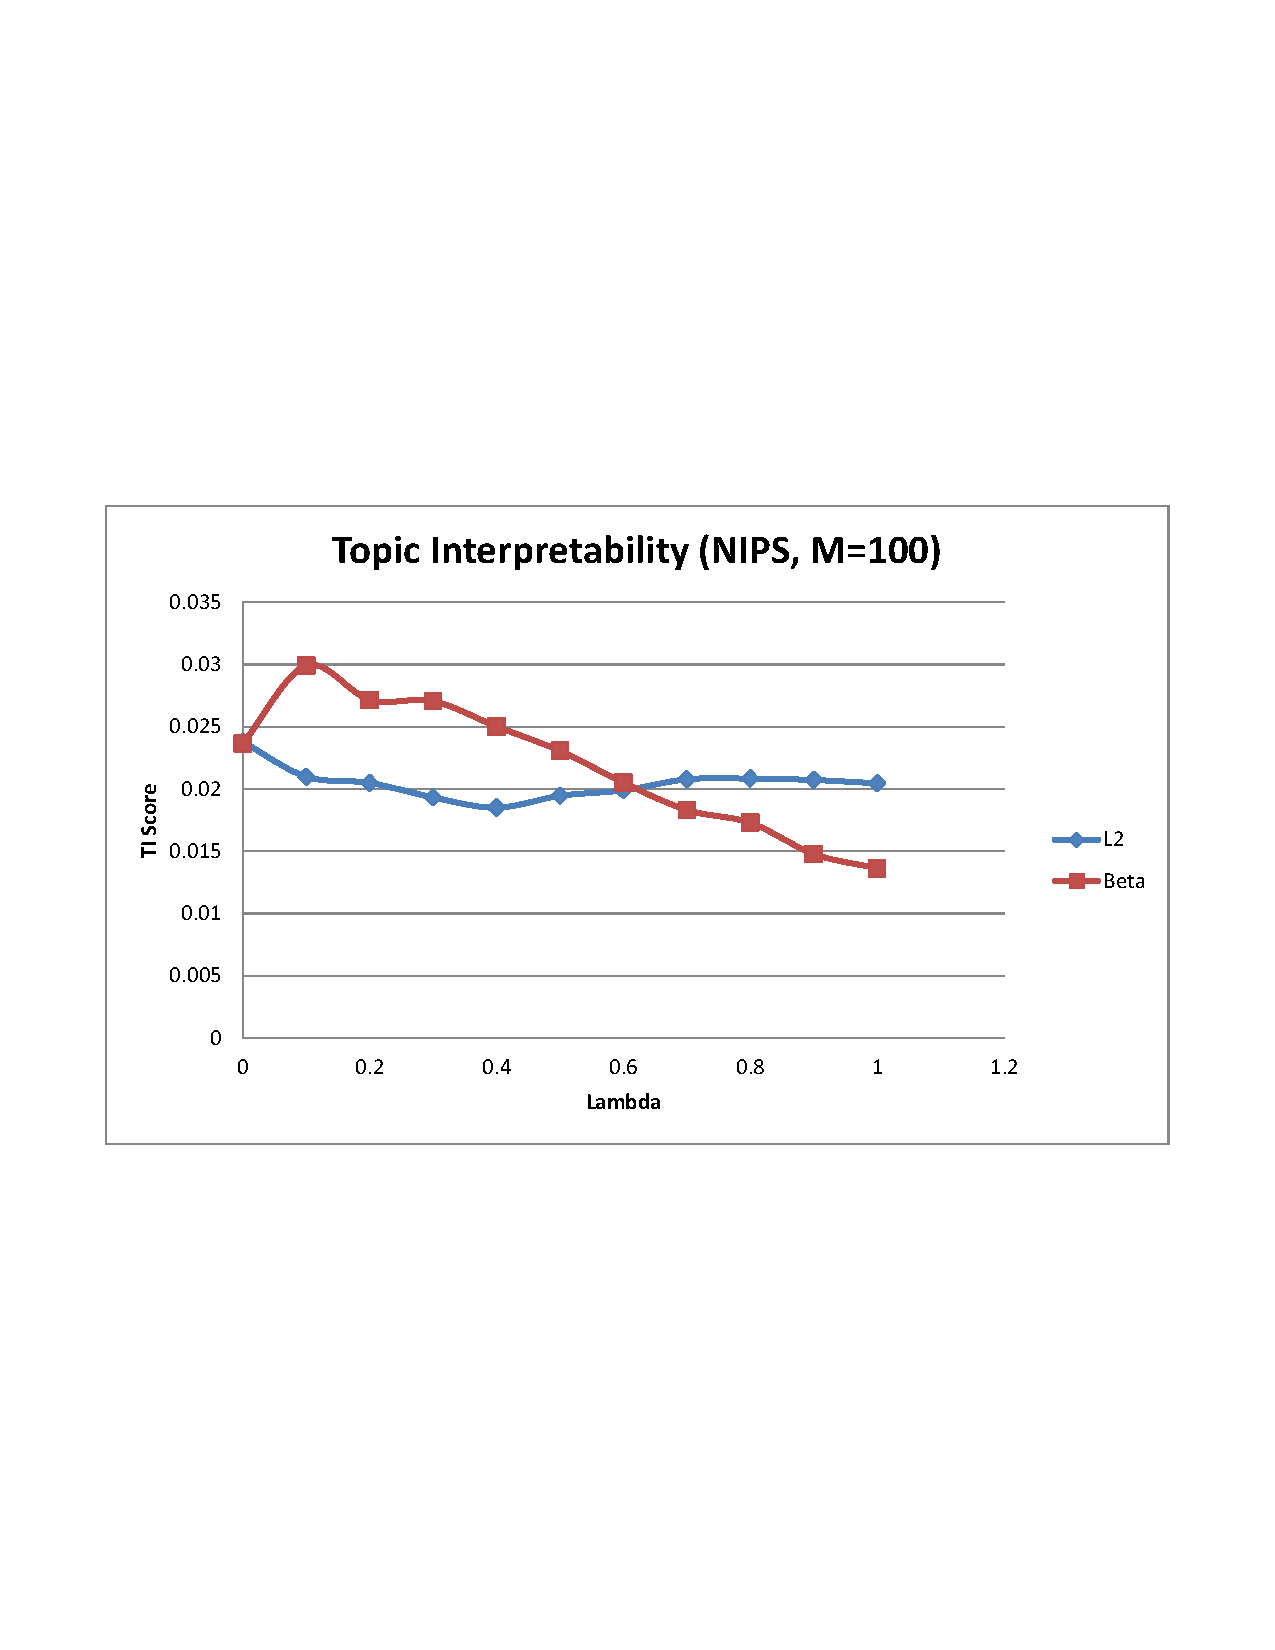
\includegraphics[width=0.7\linewidth]{figures/NIPS_M_100_TI.pdf}
\end{figure}
\vspace{-0.1in}
\begin{itemize}
\item L2 Norm performs worse than original {\bf anchor} on TI score
\item Beta Norm performs better when $\lambda=0.1$ than original {\bf anchor}
\item TEST set, {\bf anchor} TI = 0.0252; Beta Norm TI = 0.0256
\end{itemize}

\end{frame}

\begin{frame}
\frametitle{NIPS Results: Topics}

\begin{figure}
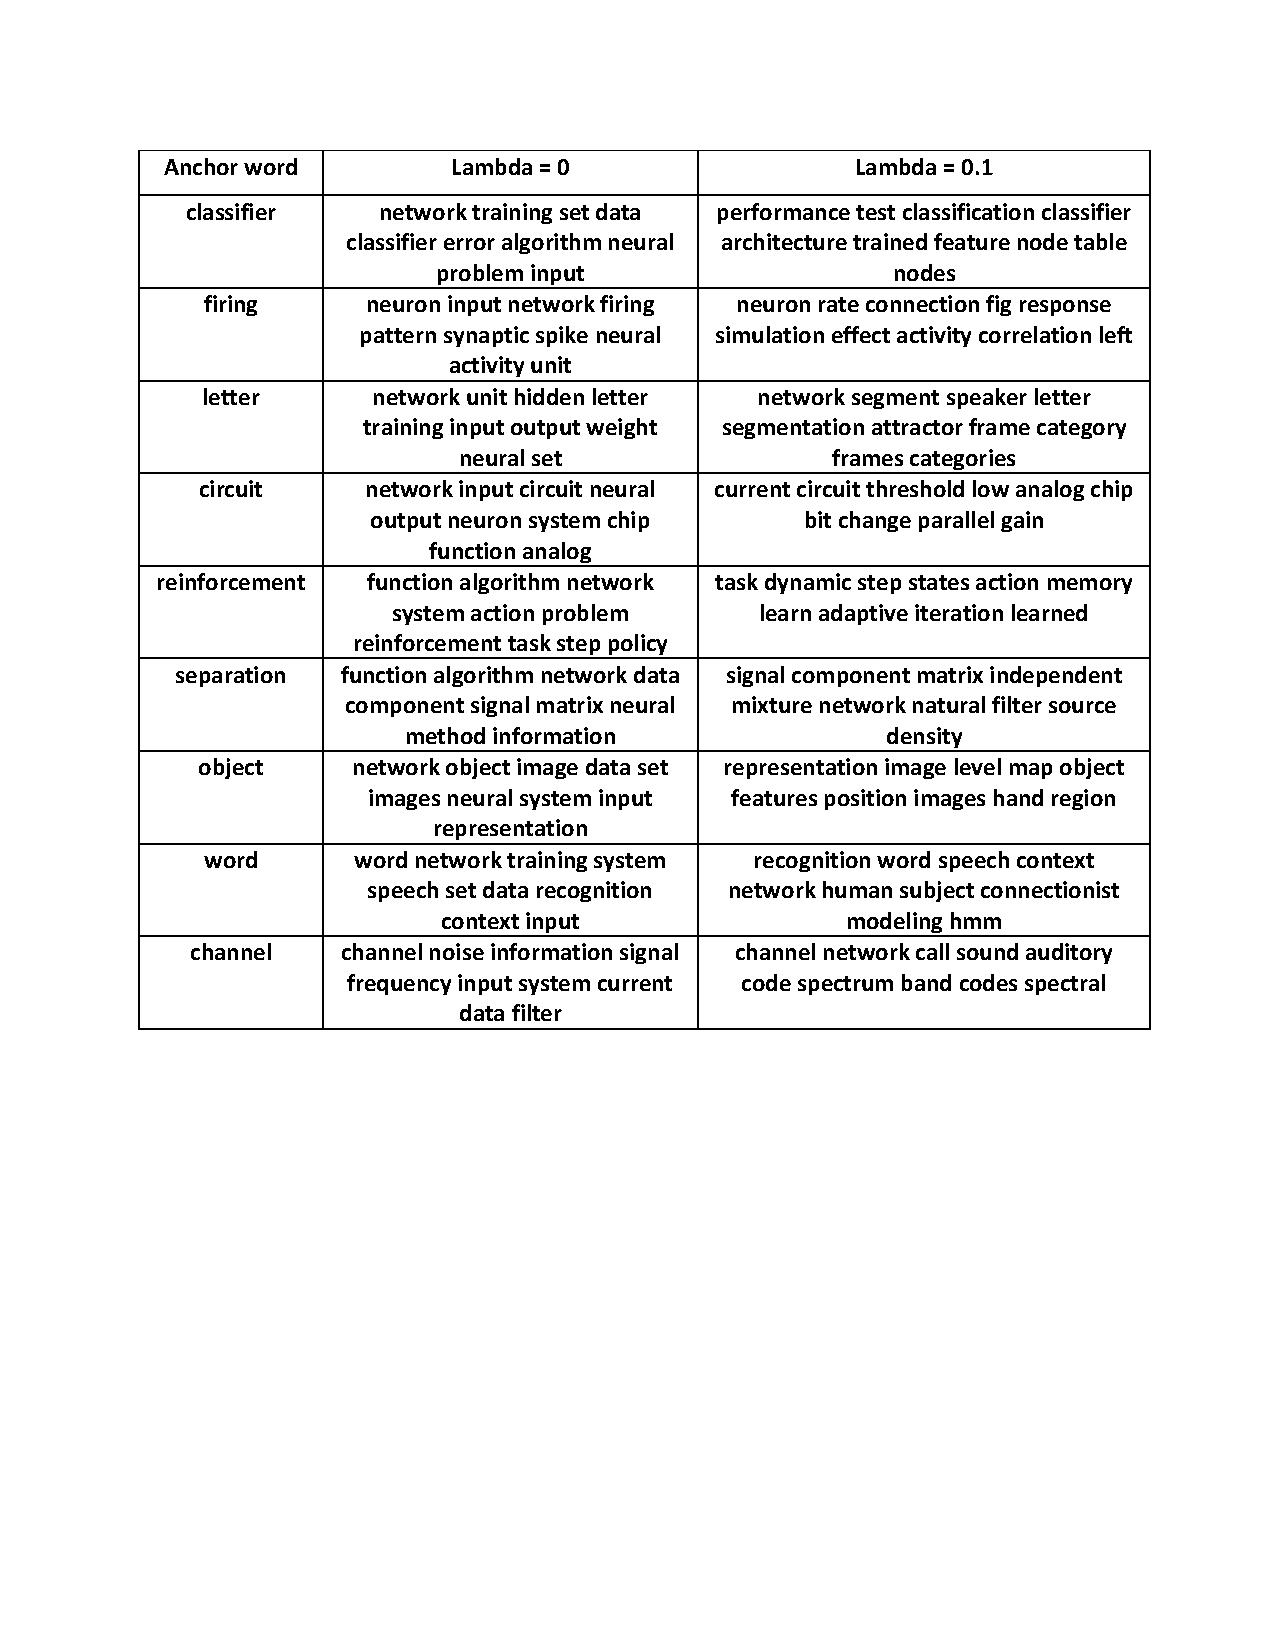
\includegraphics[width=0.7\linewidth]{figures/NIPS_Beta_0_1.pdf}
\end{figure}

\end{frame}


\begin{frame}

\frametitle{20News Results: Tuning Set, M=700}

\begin{figure}
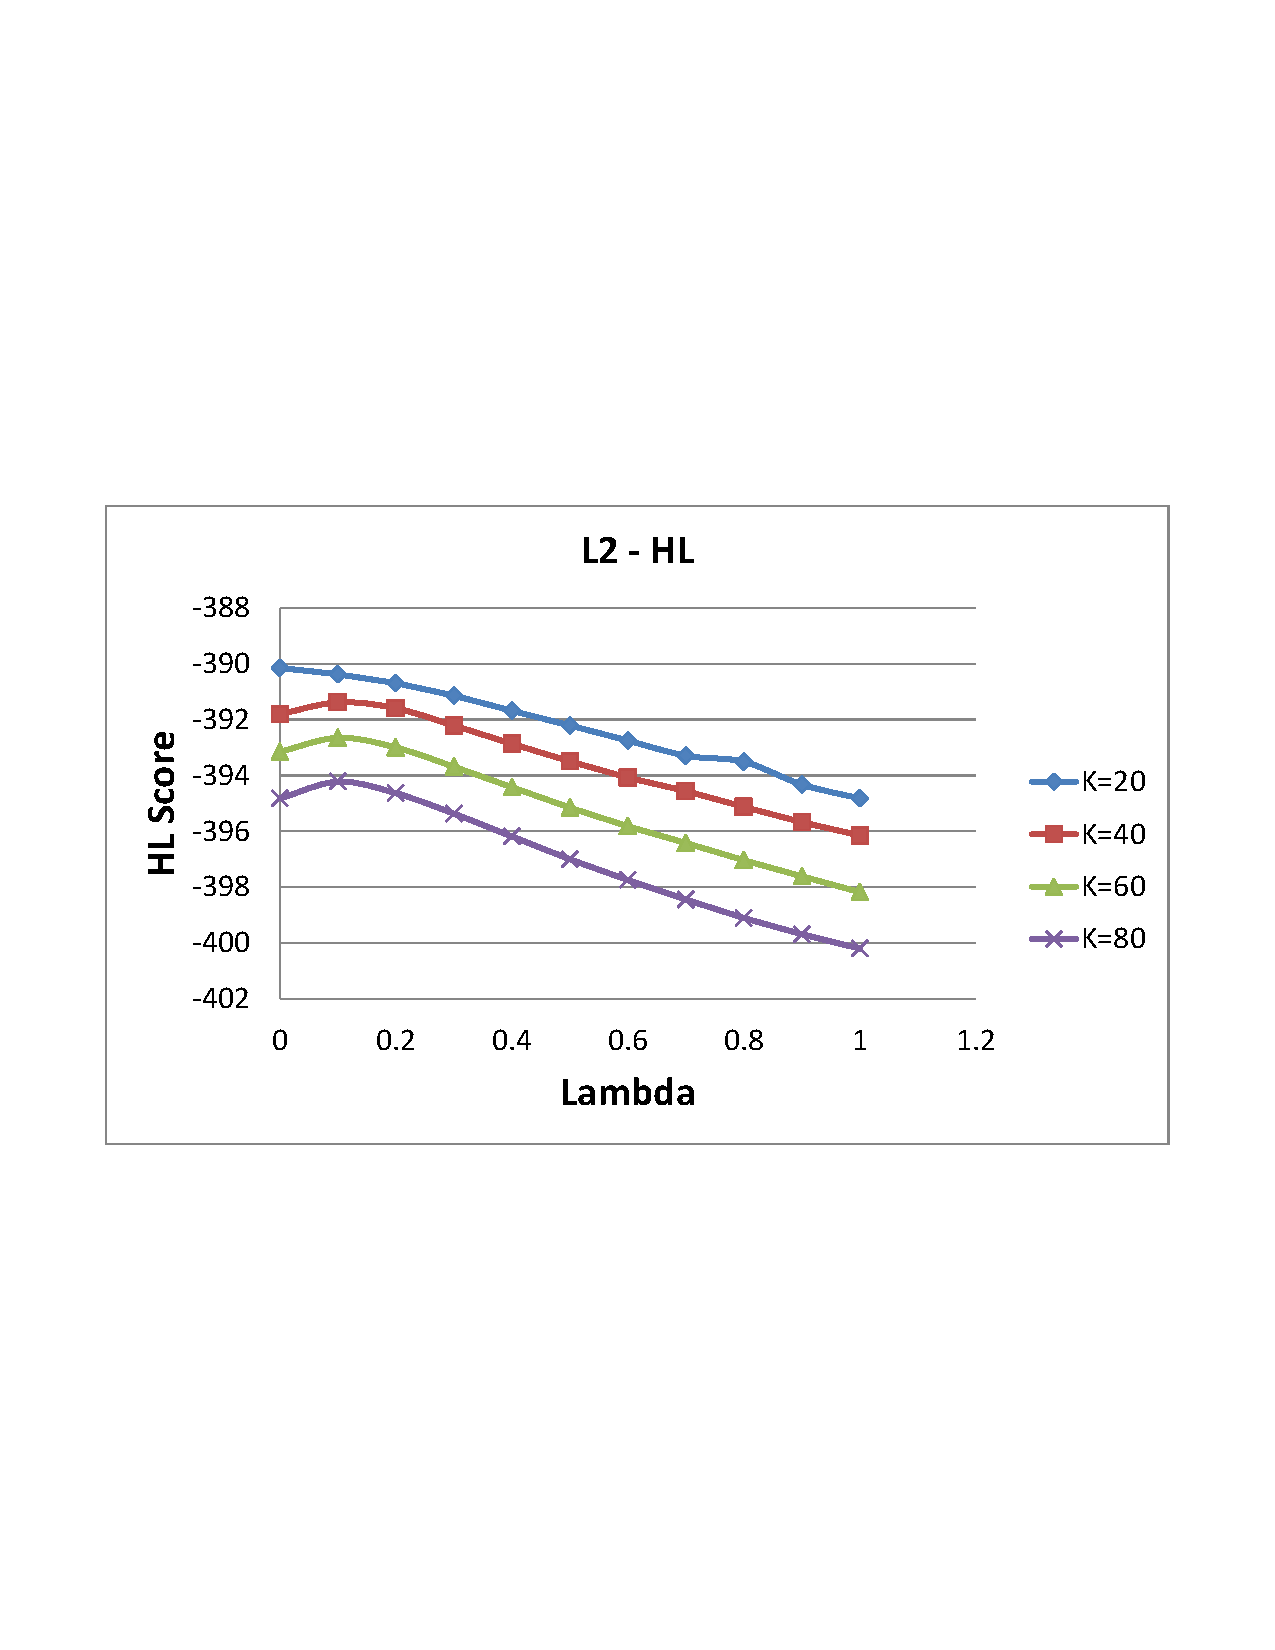
\includegraphics[width=0.7\linewidth]{figures/20news_700_Likelihood.pdf}
\end{figure}
\vspace{-0.1in}
\begin{itemize}
\item L2 Norm performs better than original {\bf anchor} when K=40,60,80 on held-out score
\end{itemize}
\end{frame}

\begin{frame}

\frametitle{20News Results: Tuning Set, M=700}

\begin{figure}
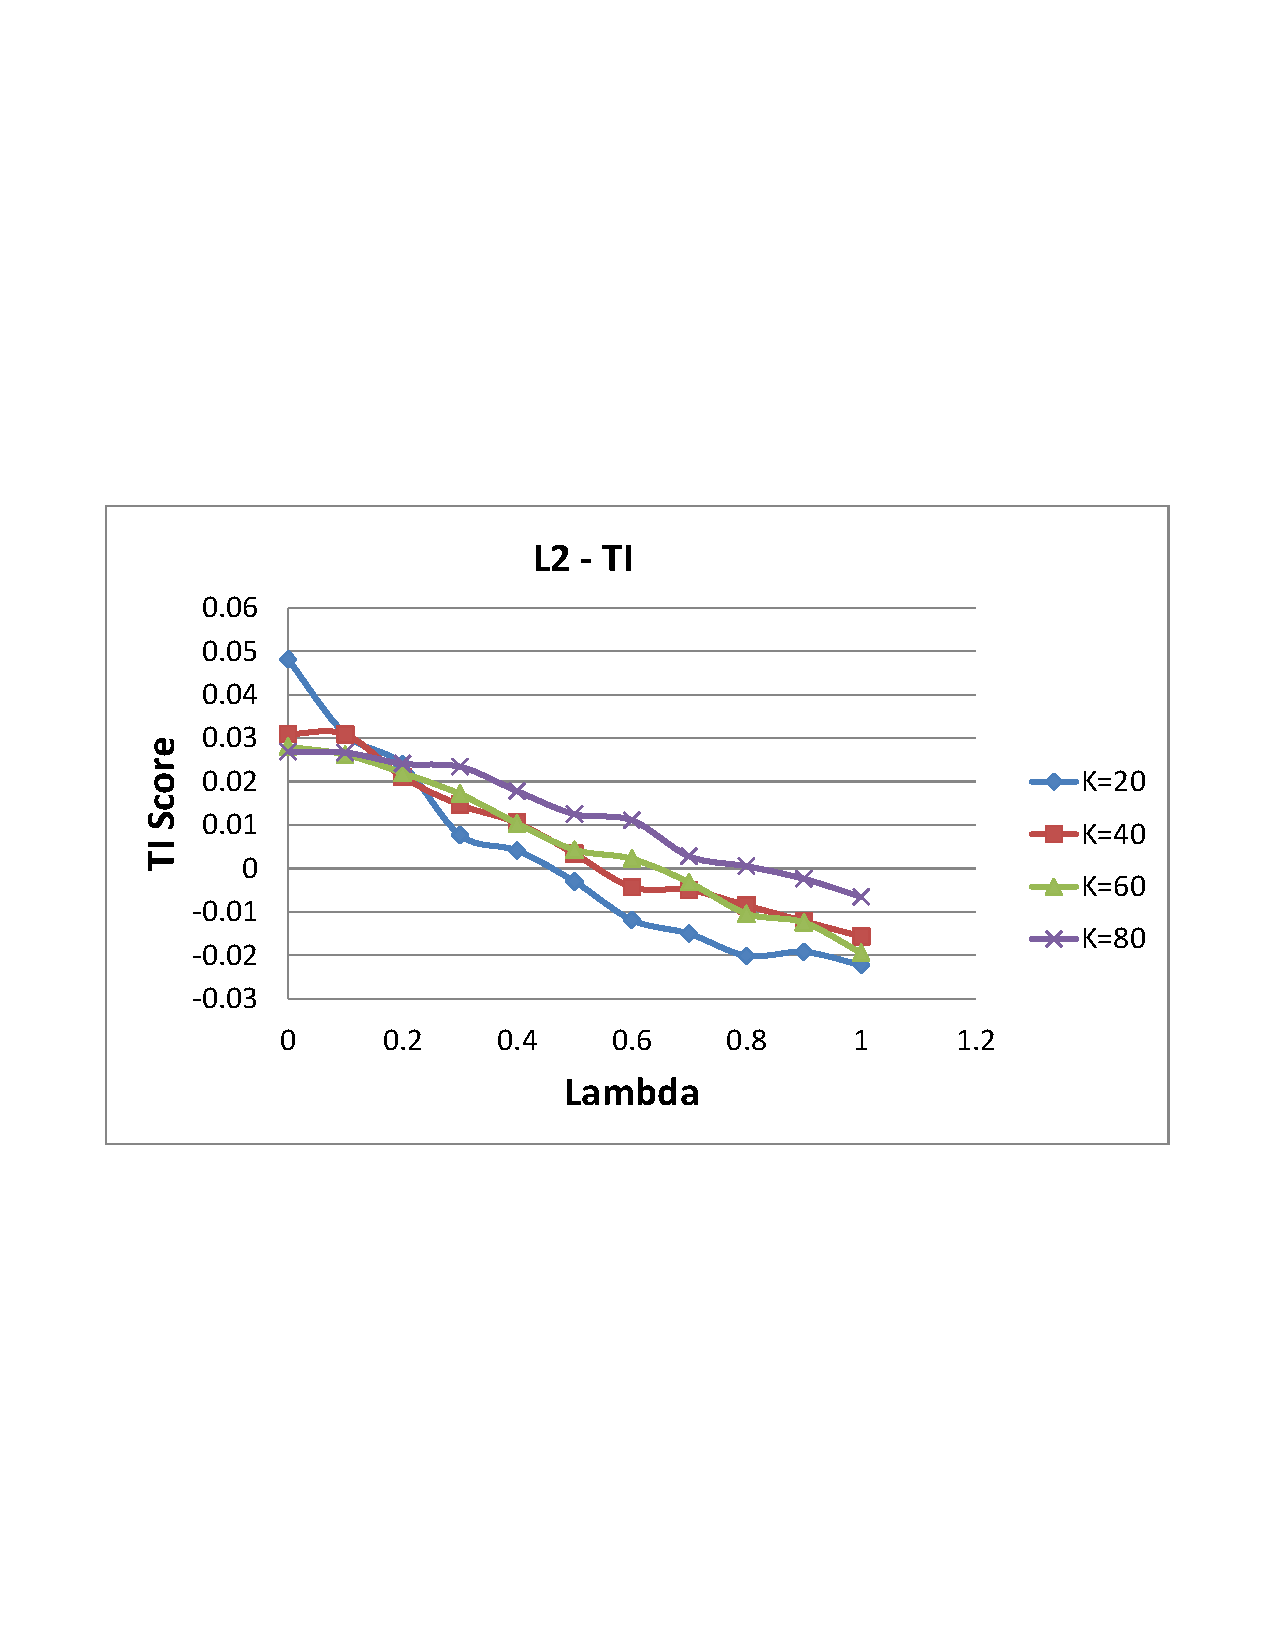
\includegraphics[width=0.7\linewidth]{figures/20news_700_TI.pdf}
\end{figure}
\vspace{-0.1in}
\begin{itemize}
\item L2 Norm performs worse than original {\bf anchor} on TI score
\end{itemize}
\end{frame}

\begin{frame}
\frametitle{20News Results: Topics}

\begin{figure}
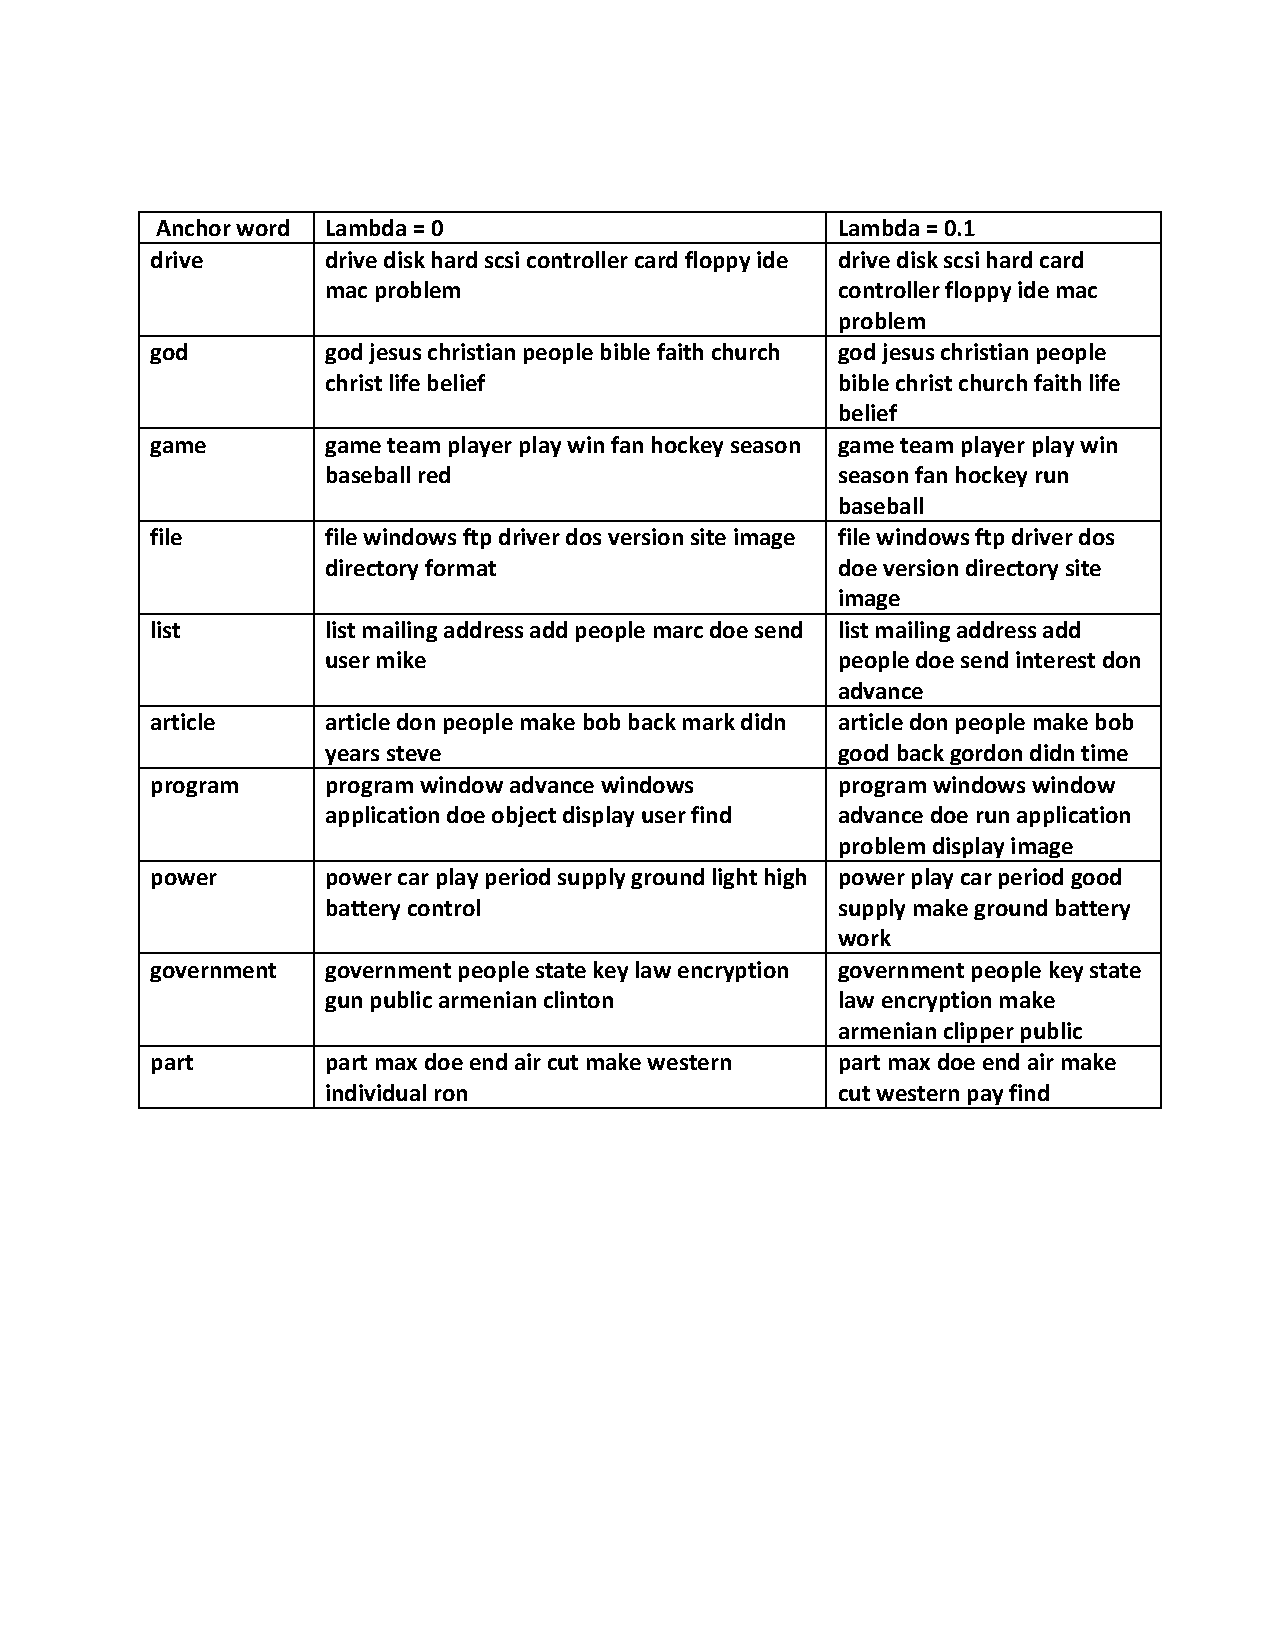
\includegraphics[width=0.7\linewidth]{figures/20news_L2_0_1.pdf}
\end{figure}
\end{frame}


\begin{frame}

\frametitle{20News Results: $\lambda = 0$, Tuning Set, various M}

\begin{figure}
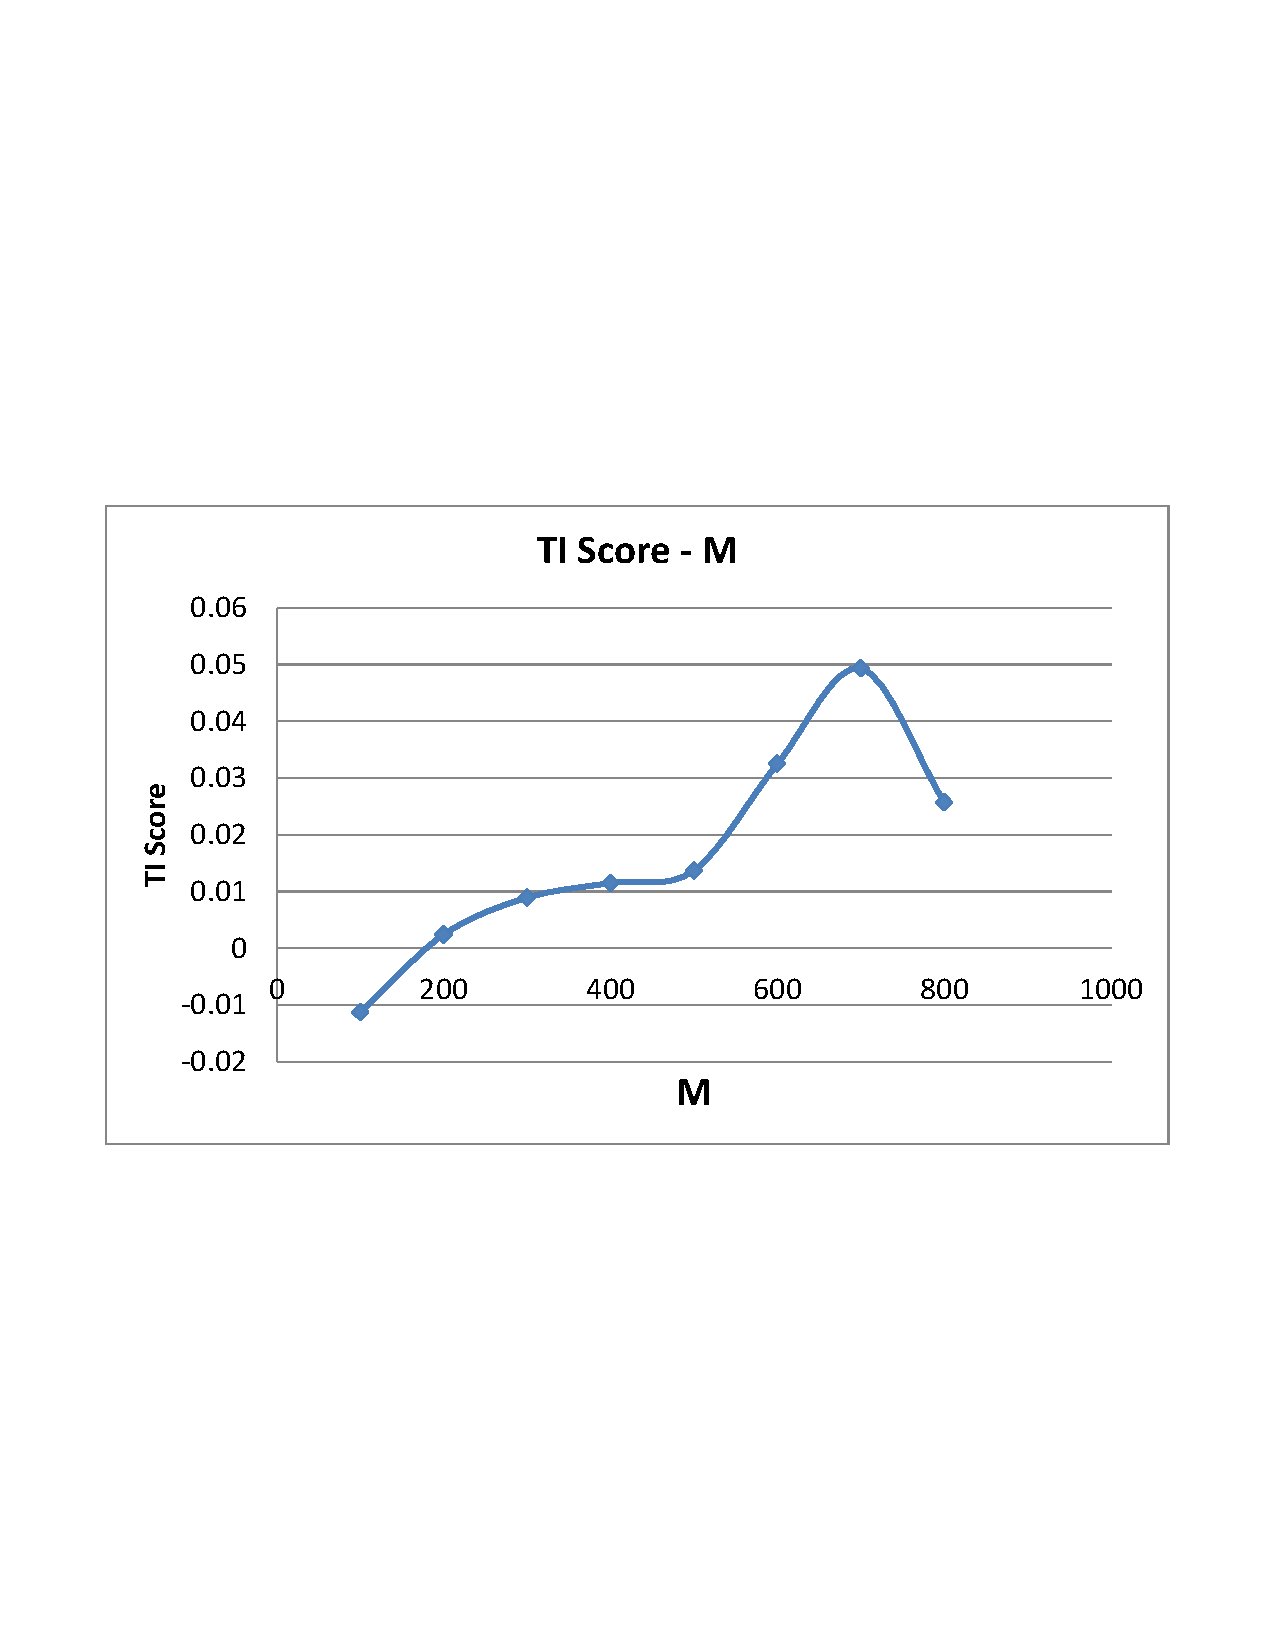
\includegraphics[width=0.7\linewidth]{figures/20news_M_TI_chart.pdf}
\end{figure}
\vspace{-0.1in}
\begin{itemize}
\item {\bf anchor} algorithm is very sensitive to how we select anchor word candidates
\item Using beta norm, $M=700$ achieved the best TI score
\end{itemize}

\end{frame}

\begin{frame}
\frametitle{Topics Comparison with Different M}

\begin{figure}
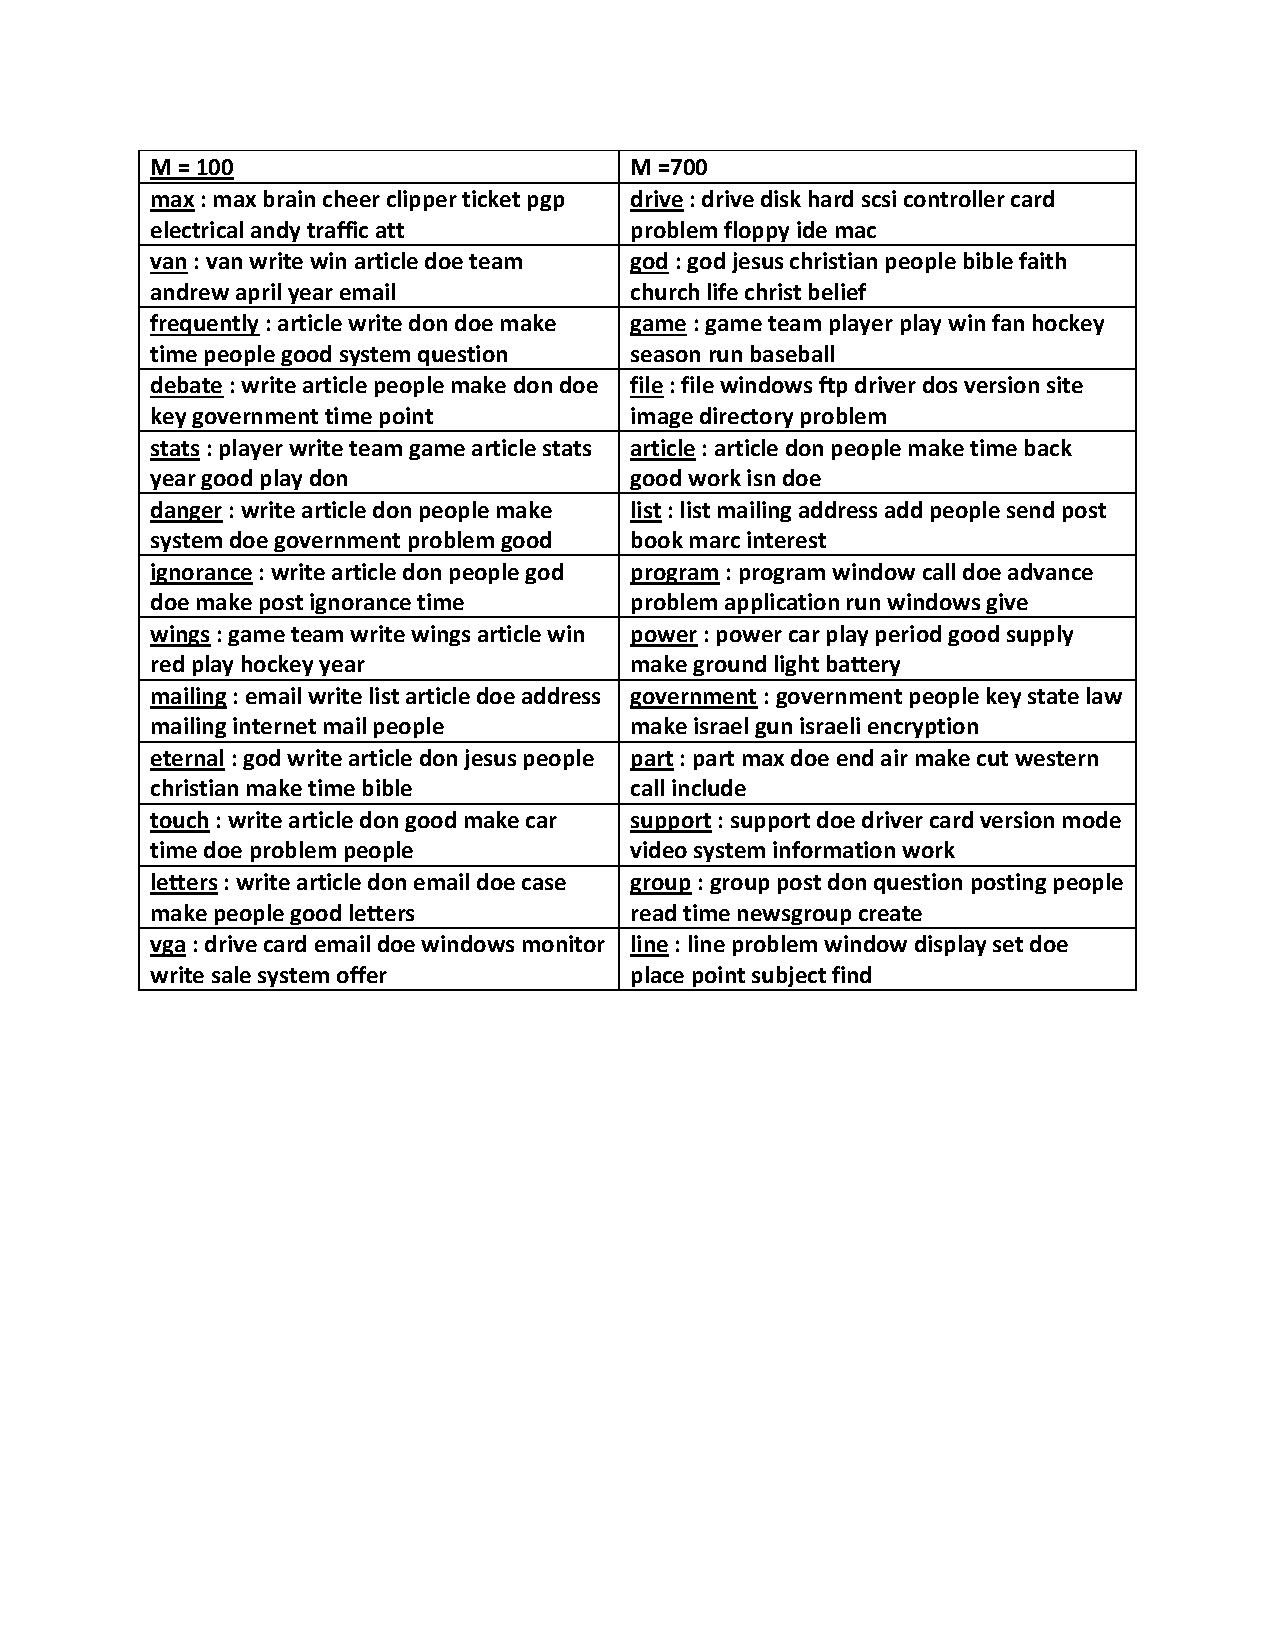
\includegraphics[width=0.7\linewidth]{figures/M_100_700_topics.pdf}
\end{figure}

\end{frame}

\begin{frame}
\frametitle{Conclusion}
\begin{itemize}
\item Introduced different priors to spectral methods
\item Evaluated the topics using topic interprebility and held-out likelihood
\item Further improve the results by,
\begin{itemize}
\item Better extract anchor words
\item Initialization of the coefficient matrix
\end{itemize}
\item Explore the moment-based spectral learning methods (Anandkumar et al, 2012)
\end{itemize}

\end{frame}

\end{document}
